\documentclass[floatfix, twocolumn, aps, prl]{revtex4-1}
\usepackage[utf8]{inputenc}
\usepackage{mathtools}

\newcommand{\avg}[1]{\langle#1\rangle}

\begin{document}
\title{Exclusivity graph approach to Instrumental inequalities}
\author{Davide Poderini}
\affiliation{Dipartimento di Fisica, Sapienza Universit\`{a} di Roma,
Piazzale Aldo Moro 5, I-00185 Roma, Italy}
\begin{abstract}
    \ldots
\end{abstract}

\maketitle

\section*{Instrumental causal structure}
\begin{figure}[h]
    \centering
    \parbox{.4\columnwidth}{
        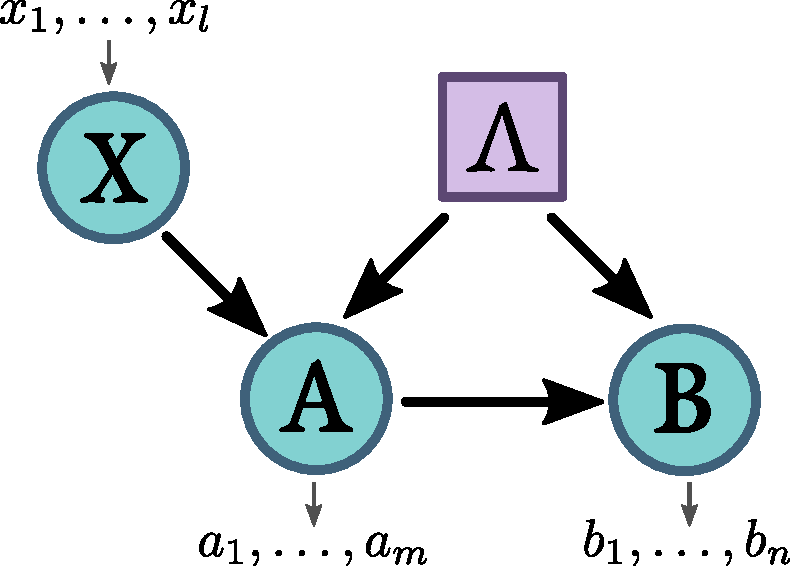
\includegraphics[width=.4\columnwidth]{images/instdag.pdf}
        \caption{The DAG representing a general Instrumental scenario.}
        \label{fig:instdag}
    }
    \qquad
    \parbox{.4\columnwidth}{
        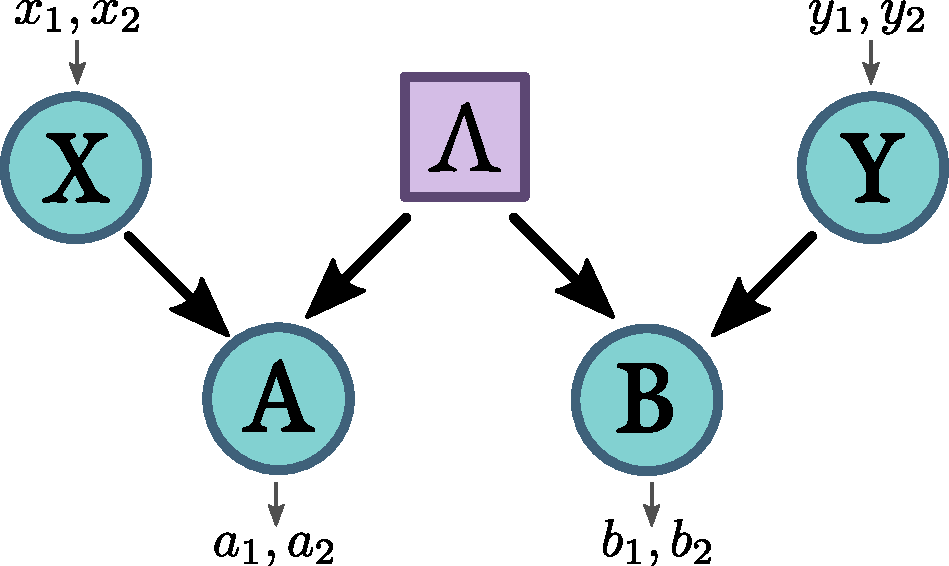
\includegraphics[width=.4\columnwidth]{images/chshdag.pdf}
        \caption{The DAG representing the CHSH scenario.}
        \label{fig:chshdag}
    }
\end{figure}

The Instrumental causal structure is a widely studied
structure both for its simplicity and commonness.
It can be described by four random variables $\Lambda, X, A, B$ where $X$ and
$\Lambda$ are independent of the others and $B$ depends on $X$ only through $A$,
as graphically depicted in fig.~\ref{fig:instdag}.

The consequences of these causal relations on the distributions of the four
variables have been throughly studied in previous works \cite{pearl1995,
bonet2001}.
Suppose that $X, A, B$ can take $l,m,n$ different values and 
call $P(a_i b_j | x_k)$ the probability that $A$ and $B$ take values $a_i$
and $b_j$ respectively, given that $X$ takes value $x_k$.
It is known that such a system must respect the following inequalities,
called \emph{Pearl's inequalities} \cite{pearl1995}:
\begin{equation}
    \sum_{j=0}^{n} P(a_i b_j|x_{k(i,j)}) \le 1
    \label{eq:pearl_ineq}
\end{equation}
for all $i \in {1,\ldots, m}$ and for all the possible functions $k(i,j)$.

In \cite{bonet2001} Bonet showed that the polytope of allowed
correlation is not tightly bounded by \emph{Pearl's inequalities}.
For instance for $(l,m,n) = (3,2,2)$ the following inequality must also be satisfied:
\begin{equation}
    P(a_1 b_1 | x_1) + P(a_2 b_2 | x_1) + 
    P(a_1 b_1 | x_2) + P(a_2 b_1 | x_2) + 
    P(a_1 b_2 | x_3) \le 2
    \label{eq:bonet_ineq}
\end{equation}
along with other similar inequalities obtained by permuting the labels of
$a_i,b_j$ and $x_k$.


These inequalities are closely related to the one presented in \cite{chaves2018}:
\begin{equation}
    -\avg{B}_{x_1} + 2 \avg{B}_{x_2} + \avg{A}_{x_1} - \avg{AB}_{x_1} +
    2\avg{AB}_{x_3} \le 3  
    \label{eq:rafael_ineq}
\end{equation}
which was experimentally violated in the same work, with a value of $3.79 \pm 0.013$.
As one can expect, with the same data we can also violate inequality
\eqref{eq:bonet_ineq} with a value of $2.159 \pm 0.005$.

A similar analysis can be done in the CHSH scenario, depicted in
fig.~\ref{fig:chshdag},
where all the variables are dichotomic.
Hence we have the notorious inequality:
\begin{equation}
    \avg{A_1B_1} + \avg{A_1B_2} + \avg{A_2B_1} - \avg{A_2B_2} \le 2
    \label{eq:chsh_ineq}
\end{equation}

As was pointed out in \cite{himbeeck2018} these two scenarios (CHSH and the Instrumental)
are related: the two quantum violations can be
seen as a consequence of one another.
Indeed if we think of the Instrumental scenario as a restricted CHSH,
where we postselect in the case of $Y = A$, and we augment the variable $X$ with
an additional value $x_3$ as described in \cite{himbeeck2018}.
From this analysis the maximum quantum violation is $(3 + \sqrt{2})/2$.

\begin{figure}[h]
    \centering
    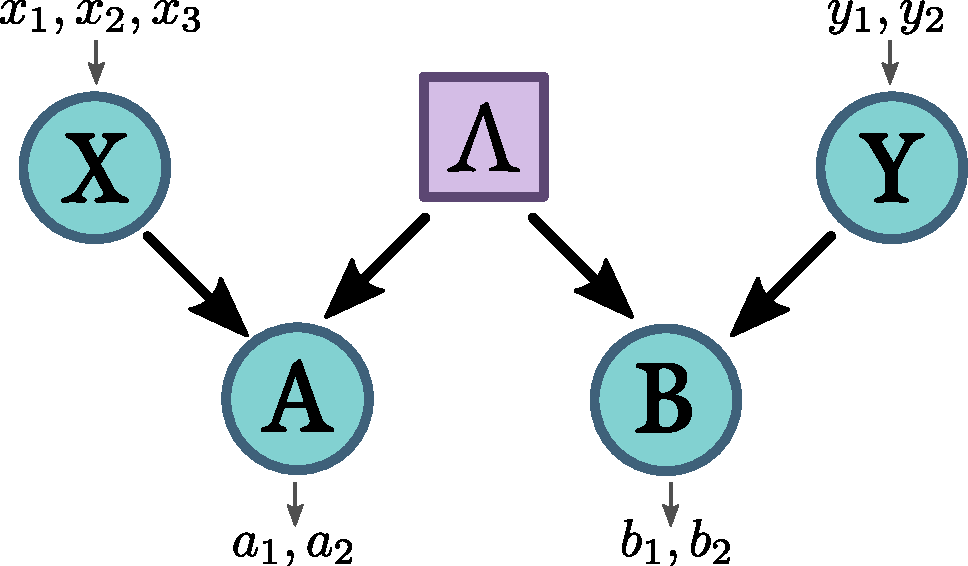
\includegraphics[width=.7\columnwidth]{images/genchshdag.pdf}
    \caption{A generalization of the CHSH DAG.}
    \label{fig:genchshdag}
\end{figure}
This can be verified experimentally provided we have an apparatus capable of
reproducing the causal structure depicted in fig.~\ref{fig:genchshdag} i.e. a CHSH scenario
where $X$ can take 3 possible values, as the apparatus presented in
\cite{chaves2018}.
Taking advantage of this we can violate all three inequalities
\eqref{eq:bonet_ineq}, \eqref{eq:rafael_ineq} and \eqref{eq:chsh_ineq} with the same set of
data:
\begin{enumerate}
    \item To violate the Instrumental inequalities we postselect in the case
        $Y = A$, obtaining values $3.787 \pm 0.013$ and $2.159 \pm 0.005$ for \eqref{eq:rafael_ineq} and
        \eqref{eq:bonet_ineq} respectively.
    \item To violate the CHSH inequality we just ignore the case $X = x_3$,
        obtaining the value $2.619 \pm 0.005$.
\end{enumerate}

\section*{Instrumental and exclusivity graphs}
\begin{figure}[h]
    \centering
    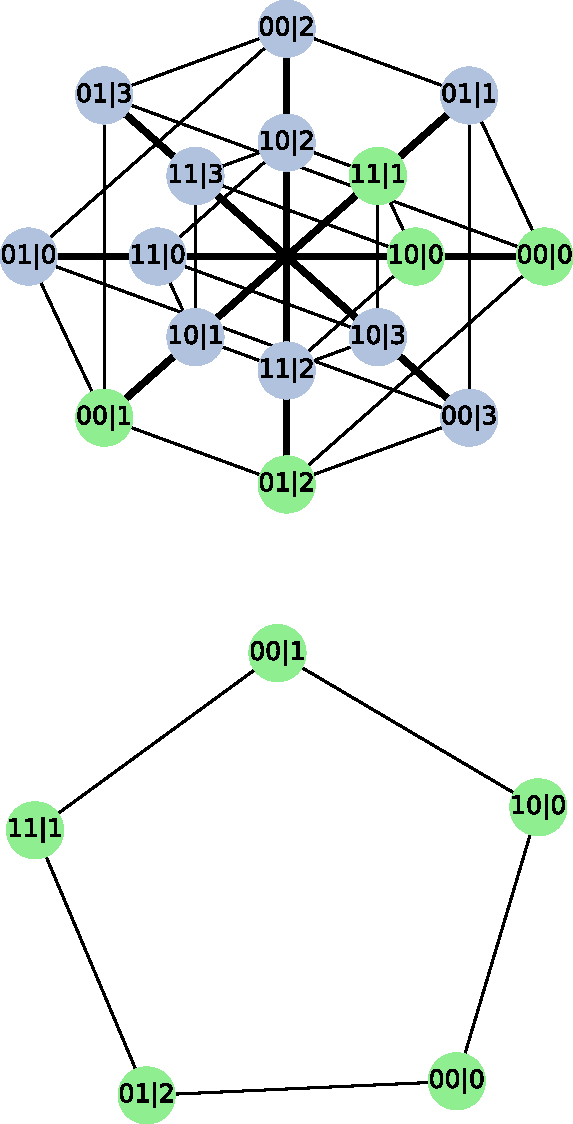
\includegraphics[width=.8\columnwidth]{images/instrumental_c5.pdf}
    \caption{The exclusivity graph of the bonet inequality.}
    \label{fig:bonetexc}
\end{figure}
The exclusivity graph method was primarly developed to study
non-contextual inequalities and obtain their quantum violation
\cite{cabello2014}. % TODO altre
In this formalism every possible event, i.e. every possible set of outcomes and
settings, is associated to a vertex in a (undirected) graph.
Two vertices are then connected by an edge if and only if they are exclusive,
i.e. if exists a measurement that can distinguish between them. % TODO espandi

Interestingly many known results about the instrumental scenario, including the
inequality \eqref{eq:bonet_ineq}, can also be obtained using this formalism.
Restricting for the moment to the case of of dichotomic observables ($n=m=2$),
we label as $p(ab|x)$ with $a, b \in \mathcal{A} = \mathcal{B} = \{0,1\}$ and $x \in
\mathcal{X} = \{0,\ldots,l\}$, the probability of having outcomes $a$ and $b$ with setting $x$. 
To obtain the exclusivity structure of the events in the instrumental scenario
we follow \cite{bonet2001}, and we say that two events $ab|x$ and $a'b'|x'$ are \emph{not} exclusive
if there exists two functions $f:\mathcal{X} \rightarrow \mathcal{A}$ and
$g:\mathcal{A} \rightarrow \mathcal{B}$ such that:
\begin{align}
    a = f(x) \quad\text{and}\quad a'=f(x')\\
    b = g(a) \quad\text{and}\quad b'=g(a')
    \label{eq:non_exclusivity_condition}
\end{align}
and exclusive if these two function do not exist.
Using this method we can construct the exclusivity graph for various $l$,
shown in figure \ref{fig:instrumental_exgraphs}, and use the methods described
in \cite{cabello2014} and \cite{rabelo2014} to obtain classical and quantum
bounds for several inequalities in the instrumental scenario. 
\begin{figure*}[h]
    \centering
    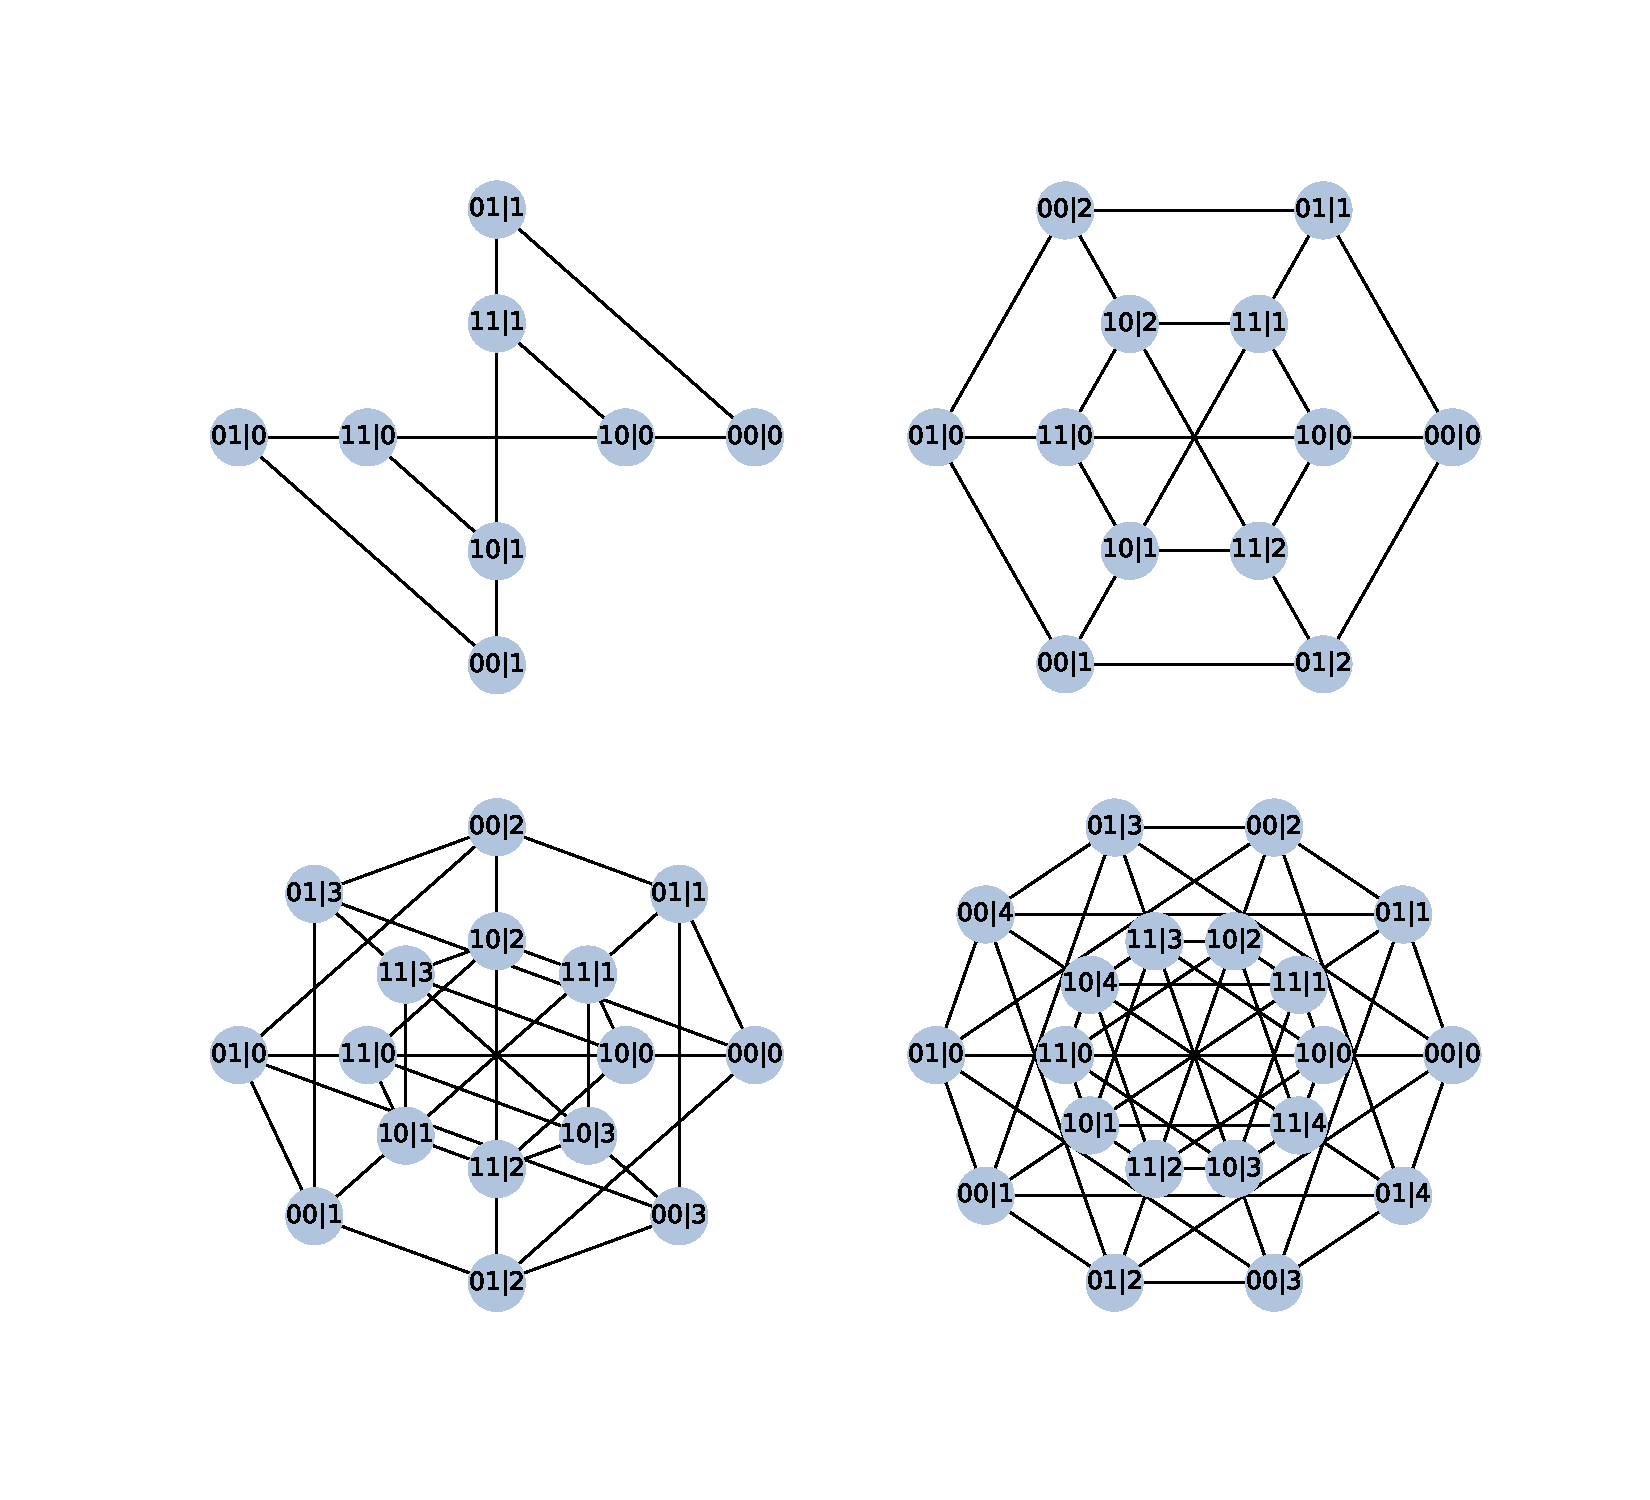
\includegraphics[width=.9\textwidth]{images/instrumental_exgraph.pdf}
    \caption{The exclusivity graph for the instrumental scenario for $l=2,3,4,5$
    from top left to bottom right.}
    \label{fig:instrumental_exgraphs}
\end{figure*}

First, using the result in \cite{cabello2014} we immediately obtain the result
that there is no quantum violation in the case of $l=2$, since the corresponding
exclusivity graph (and its complement) does not contain any odd cyclic graph
with more than $5$ vertices.  

For $l\ge3$ instead we see that there is a violation for the inequality \eqref{eq:bonet_ineq}, 
since it forms a $C_5$ cyclic graph, i.e. the pentagon depicted in
fig.~\ref{fig:bonetexc}, so that the classical limit would be $2$.
In this framework \eqref{eq:bonet_ineq} is analogous to the KCBS contextual
inequality.
We must notice that the quantum limit for the KCBS is $\sqrt{5}$, different
from the limit expected for the Bonet inequality found in \cite{himbeeck2018}.

\begin{thebibliography}{}
    \bibitem{pearl1995} J.Pearl, {\em On the testability of causal models with
        latent and instrumental variables}, 
        Proceedings of the Eleventh conference on Uncertainty in artificial
        intelligence. Morgan Kaufmann Publishers Inc. (1995).
    \bibitem{bonet2001} B.Bonet, {\em Instrumentality tests revisited},
        Proceedings of the Seventeenth conference on Uncertainty in artificial
        intelligence. Morgan Kaufmann Publishers Inc. (2001).
    \bibitem{chaves2018} R.Chaves, G.Carvacho, I.Agresti, V.Di Giulio, L.Aolita,
        S.Giacomini, F.Sciarrino, 
        {\em Quantum violation of an instrumental test}, 
        Nature Physics 14.3 291 (2018).
     \bibitem{himbeeck2018} T.Van Himbeeck, J.B. Brask, S.Pironio, R.Ramanathan, A.B.Sainz, E. Wolfe, 
        {\em Quantum violations in the Instrumental scenario and their relations to the Bell scenario},
        arXiv preprint arXiv:1804.04119 (2018).
         (2014). . 
     \bibitem{cabello2014} A.Cabello, S.Severini, A.Winter,
         {\em Graph-theoretic approach to quantum correlations}, 
         Physical review letters, 112(4), 040401 (2014).
%\bibitem{} , {\em },  ().
\end{thebibliography}

\end{document}
